\chapter{实例:mini-notify——代码插入与函数劫持在VxWorks中的实现}


\section{背景}

\subsection{Linux下的文件监控系统inotify介绍}

Linux 2.6内核中引入的inotify,
是一种监控文件系统变化的机制。
它通过提供一定的接口,
向用户空间报告底层文件系统发生的变化。
用户空间通过系统调用和文件IO操作,
来获取监视目标的变化情况。

\subsection{VxWorks下的dosFs文件系统}

VxWorks文件系统中的dosFs是MS-DOS兼容的文件系统,
可基于块对物理介质进行操作。
它提供极大的灵活性以满足实时应用的各种要求。
在VxWorks操作系统中,
文件系统的位置位于IO系统和驱动程序之间。
它们之间的层次结构如图\ref{iosys}所示。

\begin{figure}[h!]
    \centering
    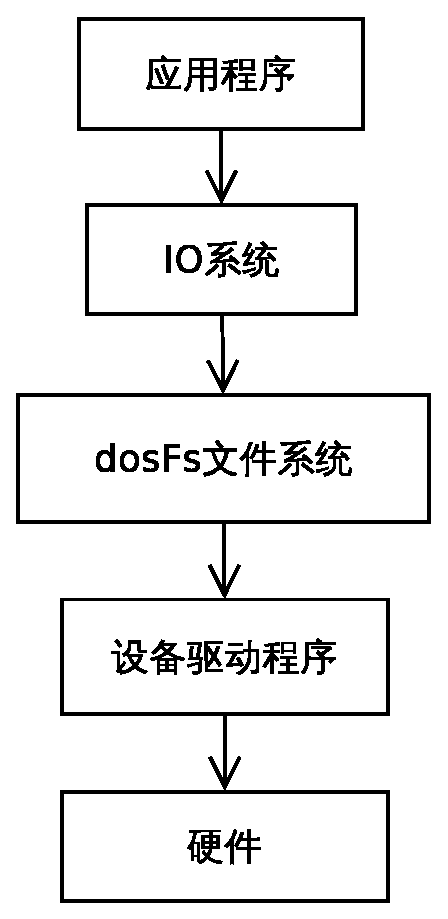
\includegraphics[width=0.21\textwidth]{figure/IOsys.eps}
    \caption{VxWorks中的IO系统图示}
    \label{iosys}
\end{figure}

具体到某个文件操作,例如open操作。
应用程序可以调用
库函数或者直接使用IO函数的时候,
他们都会调用dosFs中的dosFsOpen函数,
进而再调用驱动程序对应的函数。
最后达到访问硬件的目的。整个流程如图\ref{open}

\begin{figure}[h!]
    \centering
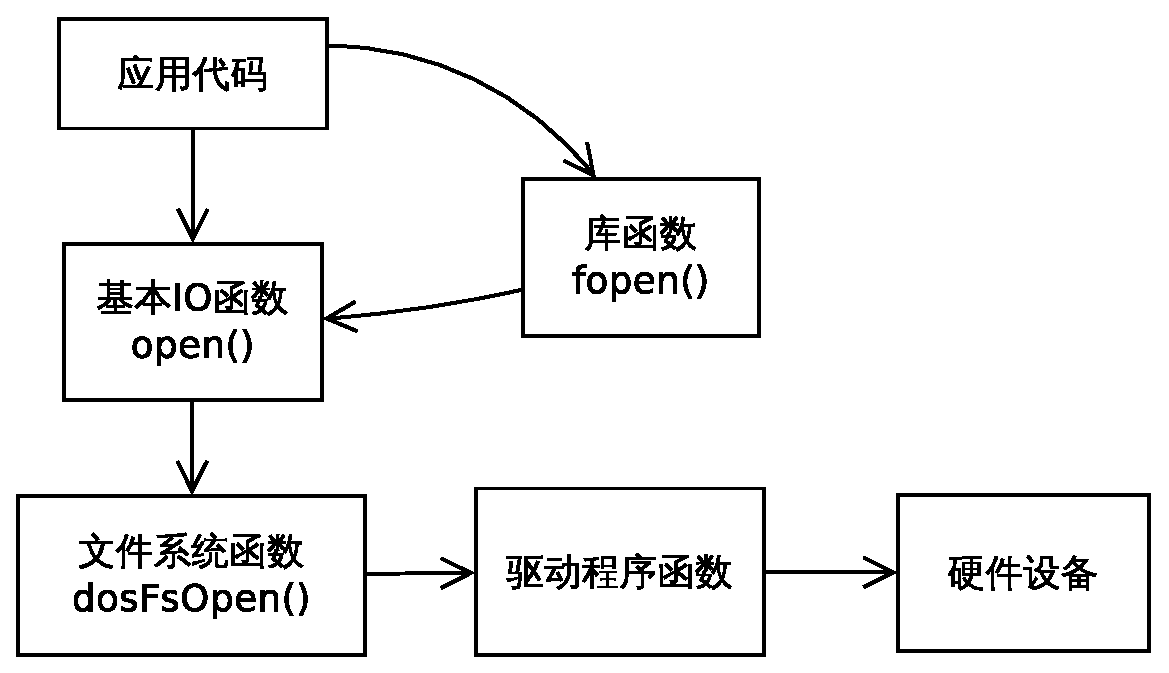
\includegraphics[width=0.58\textwidth]{figure/open.eps}
    \caption{打开一个文件的函数调用流程}
    \label{open}
\end{figure}

\section{mini-notify的目标}

mini-notify的目的是监控VxWorks下dosFs文件系统的变化,
捕获所有针对该文件系统下的任何操作,例如对文件的读和写。
并获取该操作的有关信息,
并通过一定手段向“外界”传达该信息。

mini-notify的原理如图\ref{mini0}所示

\begin{figure}[h!]
    \centering
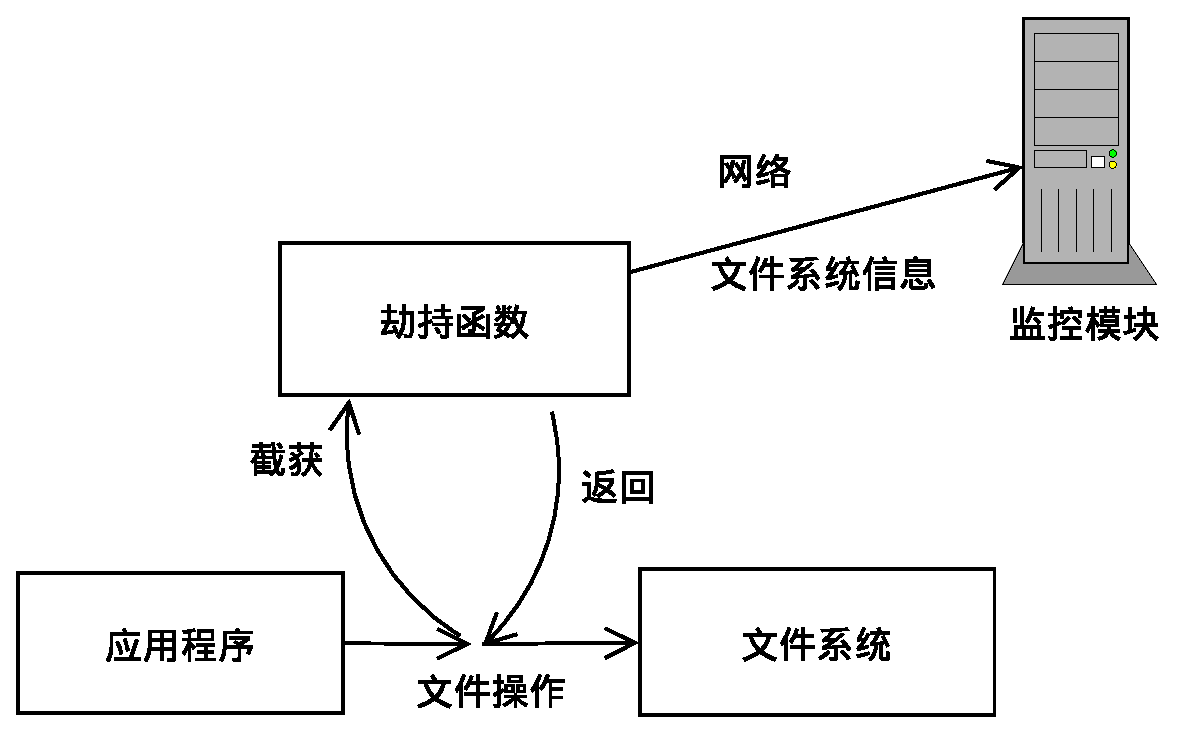
\includegraphics[width=0.59\textwidth]{figure/mini0.eps}
    \caption{mini-notify运行原理}
    \label{mini0}
\end{figure}

其中,mini-notify需要截获的文件系统操作包括:

\begin{itemize}
  \item open
  \item close
  \item read
  \item write
  \item create
  \item delete 
\end{itemize}

mini-notify需要截获并向外界监控系统报告的信息有:

\begin{itemize}
  \item 文件操作的名称(例如:read)
  \item 文件操作的具体路径(例如:/DOS/test)
  \item 系统的当前时间
\end{itemize}


\section{环境搭建与配置}

为了把精力集中于二进制层面的插入和劫持工作,
而不是目标版的连接与调试,
我们使用Vmware虚拟机来运行一个VxWorks操作系统。
这意味着我们只需要一台x86的PC就可以完成所有工作。
然而实际上我使用了两个平台:
\begin{itemize}
  \item 一台x86的Linux机器用于修改VxWorks系统映像。
  \item 一台x86的Windows机器用于运行Tornado和Vmware。
\end{itemize}

\subsection{Linux主机}

Linux主机的环境主要为我的修改工作
提供便利的工具,特别是一些GNU实用工具,
例如readelf和objdump。

安装的Linux发行版为Ubuntu 13.10的32位版本,Linux内核版本为3.11。

\subsection{Windows主机与VxWorks虚拟机}

Windows主机的主要任务包含以下几点:

\begin{itemize}
  \item 运行Tornado 2.2,生成引导程序和VxWorks系统镜像。
  \item 运行FTP Server,供目标机下载镜像。
  \item 运行Vmware 9,运行引导程序和VxWorks系统镜像。
  \item 运行Target Sever,用于与目标机通信。
\end{itemize}

图\ref{win}说明了在Windows主机下
各个软件机虚拟机的运行情况。

\begin{figure}[h!]
    \centering
    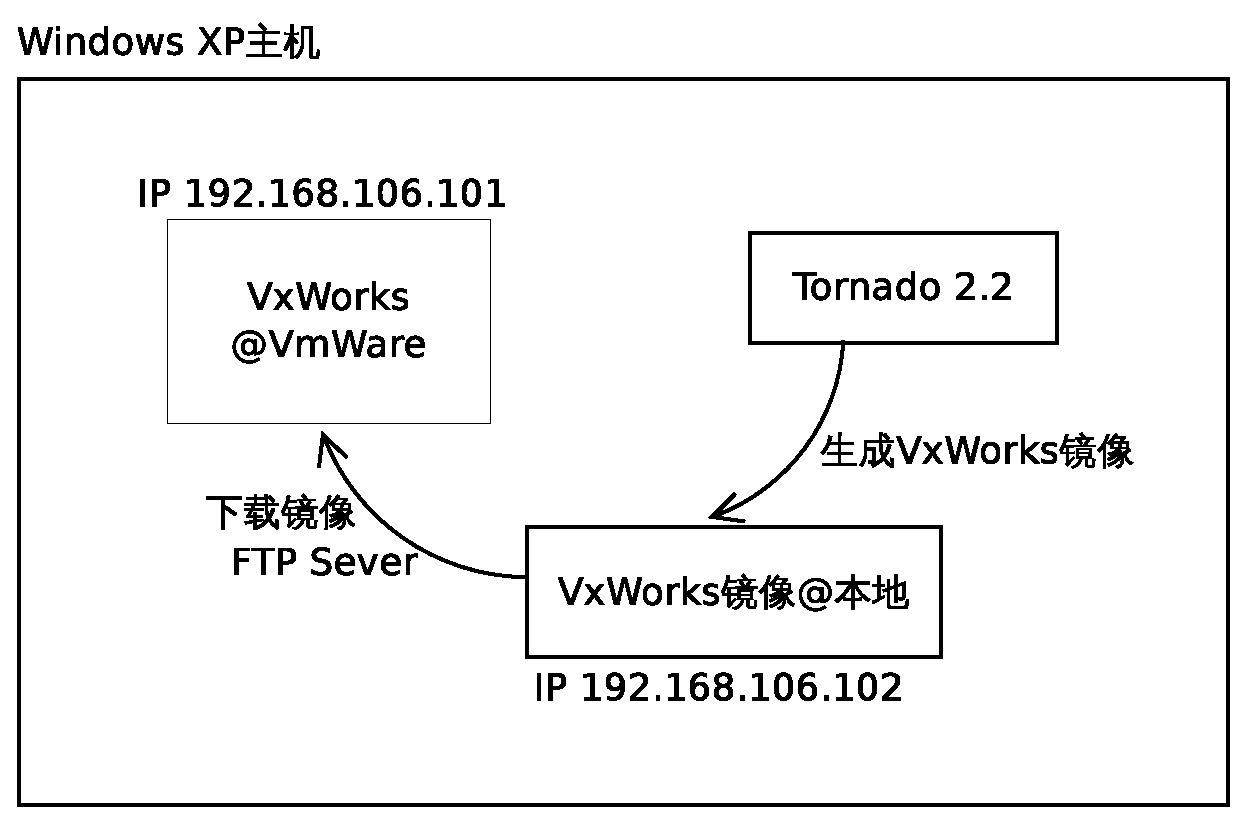
\includegraphics[width=0.68\textwidth]{figure/win.eps}
    \caption{Windows主机下的软件和虚拟机}
    \label{win}
\end{figure}

其中,在Vmware中下载VxWorks镜像,
需要首先载入bootloader,
实现的方式就不再赘述了。
在此我们可以简单地认为Tornado生成了VxWorks镜像,
而在虚拟机中即可通过FTP按照一定的路径找到该镜像
并下载。
因此,我们只需要修改该路径下的镜像文件,
并替换掉原来的文件,
当虚拟机重启后,
就会下载我们修改过的镜像文件。

\section{mini-notify方案设计}

\subsection{劫持位置选择}

我们以劫持打开文件操作为例,
阐述进行文件操作劫持的原理。
首先我们要考察劫持的位置,
即在图\ref{open}所示的哪一层的相应函数中插入跳转,
执行我们的插入代码。
我们选择对文件系统函数进行劫持,即dosFsOpen()。
因为无论上层代码使用何种方式来进行文件操作,
即无论使用哪一个库,
都会最终调用到dosFsOpen(),
dosFsOpen()函数的原型如代码\ref{open_prototype}所示。

%% open函数的原型,C代码

\begin{lstlisting}[
  language={C},
  caption={dosFsOpen()函数原型},
  label={open_prototype},
]
LOCAL DOS_FILE_DESC_ID dosFsOpen
    (
    DOS_VOLUME_DESC_ID  pVolDesc, /* pointer to volume descriptor */
    char *      pPath,  /* dosFs full path/filename */
    int         flags,  /* file open flags */
    int         mode    /* file open permissions (mode) */
    );
\end{lstlisting}

可见,dosFsOpen函数的
传入参数包含了
文件路径、文件打开的权限等信息。
这也就意味着我们可以利用插入代码获取这些信息。
而如果在更低层的驱动层来进行劫持,
文件路径等信息就消失了,
劫持工作很大程度上失去了意义。

\subsection{函数劫持方案}

为了不影响dosFsOpen的正常运行。
插入代码需要保证不污染原先的堆栈和寄存器。
我们继续使用中间层proxy作为劫持的中间代码。
控制流首先从dosFsOpen转移到proxy。
用于劫持的功能的代码则被分离出来,
单独写为一个函数,叫做hookFsOpen。
图\ref{proxy}展示了劫持dosFsOpen函数的跳转过程。

\begin{figure}[h!]
    \centering
    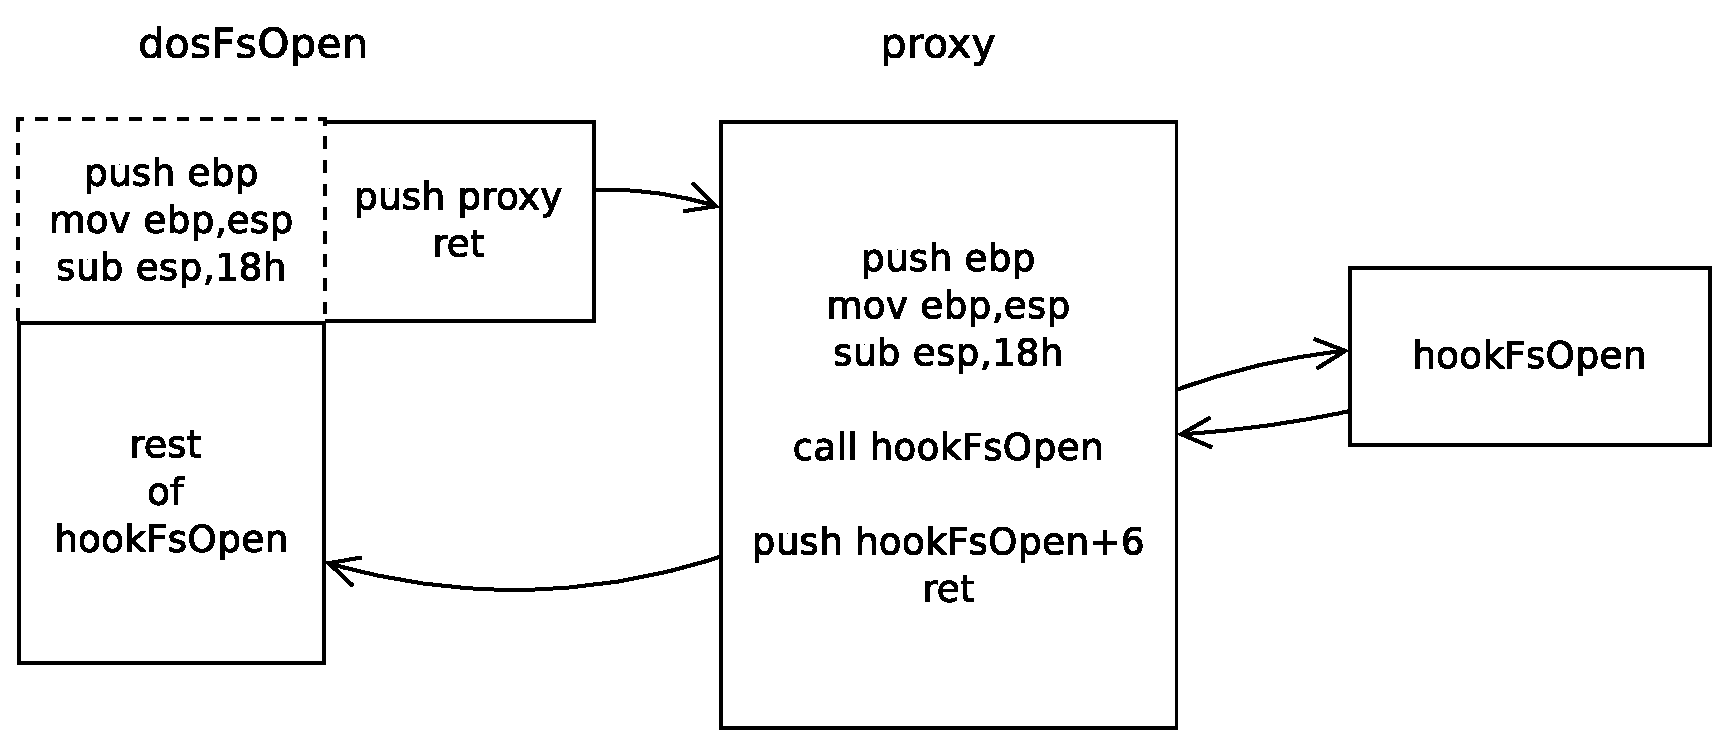
\includegraphics[width=0.76\textwidth]{figure/proxy.eps}
    \caption{劫持dosFsOpen的函数跳转流程}
    \label{proxy}
\end{figure}

我们将dosFsOpen函数开头的三条指令(位于虚线框中)替换为
右边方框的指令。
并在proxy开头补充这三条指令。
这样一来,proxy就很自然地拓展了dosFsOpen函数的空间,
可以在其中写入任何代码,
只需要在最后返回即可。
我们在proxy中使用call指令调用hookFsOpen函数,
一方面避免了在proxy中进行堆栈和寄存器的恢复;
另一方面,
我们hook函数不必真的像“插入”的函数那样小心翼翼,
担心污染了寄存器和堆栈。
总之,我们可以像编写正常的C语言函数一样,
来编写hookFsOpen()。

\subsection{代码插入方案}

在插入方案上,我们选择更简单的利用nop
指令串的方案。
在选择了插入方案和函数劫持方案的基础上,
我们来考察如何能够更加方便地插入proxy和劫持函数。

附录\ref{python}中针对VxWorks的代码插入工具,
可以以汇编代码作为输入。
我们可以将proxy和劫持函数写在一起,例如对于dosFsOpen函数来说,
对应的插入代码如代码\ref{finish}所示。

\begin{lstlisting}[
 language={[x86masm]Assembler},
 caption={为插入而准备的汇编代码},
 label={finish},
]
global _start
section .text
_start:                      ;proxy部分
    push ebp
    mov ebp,esp
    sub esp, 0x18            ; 补上dosFsOpen开头被替换的指令
    call hookFsOpen          ; 调用hookFsOpen,可通过相对寻址定位
    push dosFsOpen+6
    ret                      ; 返回至dosFsOpen第四条指令处

hookFsOpen:
    ......
    ......                   ; hookFsOpen函数体
\end{lstlisting}

这一份汇编代码中,同时包含了proxy和hookFsOpen函数。
因此对于每一个被劫持的函数,只需要使用一份汇编代码,进行一次插入即可。
此外,hook函数体使用了汇编语言中的label,proxy对它的调用可以通过label
来进行间接寻址,从而为我们节省了手动重定位的工作。

\section{mini-notify的实现}

完整的mini-notify包含
针对6项基本文件操作(create,delete,open,close,read和write)的6个劫持函数。
所有的劫持函数源代码见附录\ref{hook}。

劫持函数每次被调用,主要进行以下两个方面的工作:

1、获取和解析dosFs函数的参数;

2、使用ftp向目标机器发送相应的信息,包含操作名称,文件路径(pPath参数)和系统时间。


\section{测试与评价}

本节,我们使用插入了mini-notify的系统镜像,
运行一个简单的测试用例,
测试用例代码见代码\ref{file}。
为了更方便地获得mini-notify收集的信息,
我们将通过ftp传送改为直接在屏幕上打印。

\begin{lstlisting}[
  language={C},
  caption={operate\_file()函数源代码},
  label={file},
]
void operate_file(){
     int fd; 
     int nWritten,nRead;
     char read_buf[20]; 
     char *write_buf = "Hello dosFs!!!";

     memset(read_buf,0,sizeof(read_buf));
     fd = open("/DOSB/test1", O_CREAT | O_WRONLY, 0644);

     nWritten = write(fd, write_buf, 15);
     close(fd);
     fd = open("/DOSB/test1", O_CREAT | O_RDONLY, 0644);
     nRead = read(fd, read_buf, 20);

     printf("fd:%d,write:%d,read:%d,contains:%s\n",fd, nWritten,nRead,read_buf);
}
\end{lstlisting}


运行这一测试用例的结果如图\ref{after}所示。

\begin{figure}[h!]
    \centering
    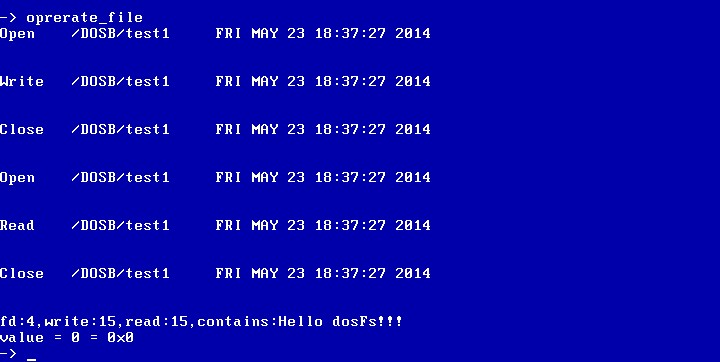
\includegraphics[width=0.85\textwidth]{figure/after.jpg}
    \caption{测试程序运行结果}
    \label{after}
\end{figure}

从该函数的输出中可以看出,
测试用例中每次调用文件操纵函数,
屏幕中都会打印一行输出,
输出的信息包含三个部分,
分别是操作的内容,目标文件路径和系统时间。

该测试用例证明mini-notify的基本功能运作正常。
然而作为一个文件监控系统而言,
mini-notify仍有很多不足之处,
下面列举出几条:

1、无法为应用程序提供接口,来由应用何时获取何种信息。而是强制地捕获文件系统信息。

2、获取的信息量有限,无法例如无法获知文件读写的内容等。

3、对于段时间内频繁的文件读写操作,mini-notify只会简单地报告信息,而不会根据时间进行合并和整理。

















